\documentclass[runningheads,a4paper]{llncs}

\usepackage{amssymb}
\setcounter{tocdepth}{3}
\usepackage{graphicx}
\usepackage{booktabs}

\usepackage{url}
% \urldef{\mailcf}\path|{berlin,borazio}@ess.informatik.tu-darmstadt.de, tobias.grosse-puppendahl@igd.fraunhofer.de|
% \newcommand{\keywords}[1]{\par\addvspace\+baselineskip
% \noindent\keywordname\enspace\ignorespaces#1}

\begin{document}

\mainmatter  % start of an individual contribution

% first the title is needed
\title{Enhancing Accelerometer-based Activity Recognition with Capacitive Proximity Sensing}

% a short form should be given in case it is too long for the running head
\titlerunning{Enhancing Accelerometer-based Activity Recognition with Proximity Sensing}
% (feature abused for this document to repeat the title also on left hand pages)
\authorrunning{Enhancing Accelerometer-based Activity Recognition with Proximity Sensing}

% the name(s) of the author(s) follow(s) next
\author{Tobias Grosse-Puppendahl\inst{1} \and Eugen Berlin\inst{2} \and Marko Borazio\inst{2} }
%\author{Author 1 \and Author 2 \and Author 3 }

% the affiliations are given next; don't give your e-mail address
% unless you accept that it will be published
\institute{
 	Fraunhofer IGD, Darmstadt, Germany\\
 	\email{tobias.grosse-puppendahl@igd.fraunhofer.de}
 	\and
 	Embedded Sensing Systems, Technische Universit\"at Darmstadt, Germany\\
 	\email{\{berlin,borazio\}@ess.tu-darmstadt.de}
}

%\institute{
	%Anonymized for review \\
	%\email{anonymous@insitution.edu}
	%\and
	%Anonymized for review \\
	%\email{anonymous@insitution.edu}
%}


\toctitle{Enhancing Accelerometer-based Activity Recognition with Capacitive Proximity Sensing}
\tocauthor{Eugen Berlin, Marko Borazio, Tobias Grosse-Puppendahl}

\maketitle
\begin{abstract}
Activity recognition with a wearable accelerometer is a common investigated research topic and enables the detection of basic activities like sitting, walking or standing. Recent work in this area adds different sensing modalities to the inertial data to collect more information of the user's environment to boost activity recognition for more challenging activities. This work presents a sensor prototype consisting of an accelerometer and a capacitive proximity sensor that senses the user's activities based on the combined sensor values. We show that our proposed approach of combining both modalities significantly improves the recognition rate for detecting activities of daily living.
\keywords{activity recognition, capacitive proximity sensors, ambient assisted living, user context}
\end{abstract}

\section{Introduction}

Persons affected from physical and mental restrictions and their care givers can profit significantly from unobtrusive activity monitoring solutions. For example, formal care givers could equip a person with a wearable activity monitoring system that evaluates the course of a disease or the influence of an adapted medication \cite{Muhlsteff2004a}. This scenario is especially relevant for people suffering from dementia who have limitations in organizing their daily activities. A simple wearable activity monitoring solution could analyze activities performed in daily life, such as drinking, eating and sleeping habits. 

Sensing a person's activity is an active research topic with a raising interest due to the advancement in mobile phone technology. These devices include multiple sensors and therefore enable the recognition of daily activities \cite{brezmes2009activity}. Current wearable activity recognition systems are able to unobtrusively capture and recognize a person's activities throughout the whole day. These systems often rely on inertial sensor data that are captured by wearable sensors embedded in a mobile device \cite{brezmes2009activity} or attached to the body \cite{Ravi2005}. Usually, single sensor modalities are used or duplicated to detect the activities. However, it is a great challenge to identify many activities just by using a single modality like the accelerometer.

Capacitive proximity sensors on the other hand can indirectly measure the distance and nature of a grounded object within reach. This means that the measurement result depends on the object's distance, its size and the material it is made of. In this work, we show that an accelerometer and a capacitive proximity sensor can be used to improve activity recognition in activities of daily living that rely heavily upon object usage. Therefore, we obtained an open-hardware and open-source wrist-worn activity data logger \cite{hedgehog} and integrated a capacitive proximity sensor into its wristband. 

There are several intuitive examples for which a combination of accelerometer-based activity recognition with a capacitive proximity sensor reveals its strength. For example, it may be conducted which material is placed underneath the wristband. The capacitive proximity sensor would return a different measurement result for a hand placed on a couch covered with fabric than a hand placed on a wooden table. Moreover, the approximate distance from the wristband to objects can be exploited to identify activities like grasping into a locker or a refrigerator to prepare food.

The remainder of this paper is structured as follows: First, Section \ref{sect:related} is dedicated to related work work in activity recognition, in particular considering approaches with multiple sensing modalities. Section \ref{sect:hardware} presents the hardware based on which a wrist-worn sensor prototype was built, fusing an inertial data logger and a capacitive sensor integrated into a wristband.
The experimental setup, the scenario with daily activities and the activity recognition evaluation results, showing the performance boost of the capacitive sensor unit, are given in Section \ref{sect:experiment}. The paper is wrapped up with a conclusion enumerating the findings of the evaluation, as well as pointing out future research potential.

\section{Related Work}
\label{sect:related}
%%%%%%%%%%%%%%%%%%%%%%%%%%%%%%%%%%%%%%%%%%

Activity recognition research relying on wearable sensors mostly considers inertial data from the participants body to infer performed activities, such as in the works of \cite{Ravi2005,Bao2004,Srinivasan2010,Amft2005}. The acceleration data is often augmented with data from sensors such as gyroscopes \cite{Holleczek_2010}, magnetometers \cite{Altun_2010}, ambient light \cite{Borazio2012} or ambient and skin temperature \cite{Krause_2003}, aiming to extract a more detailed environmental user context. In \cite{wyss2010recognition}, the authors use heart rate information as an addition to the accelerometer data to detect activities like lifting and lowering loads or even digging. In \cite{Ward_2006}, workshop assembly activities are detected by augmenting acceleration sensors with microphones.

The works of Fishkin et al. \cite{Fishkin_2005} and Patterson et al. \cite{patterson2005fga} show that detecting touched and used objects can be very helpful for activity recognition. By using RFID readers that are embedded in gloves or bracelets at the wrist and RFID tags attached to various objects of interest, one can detect the object grasped and used by the user, thus aiding the activity recognition in various application scenarios, such as activities of daily living \cite{phealth:maja} and \cite{Philipose_2004}, activity tracking in car manufacturing \cite{Stiefmeier08}, or household and gardening activities \cite{berlin_laerhoven_tei_2010}. 

Our approach to enhance the inertial data from a wearable sensor is comparable to the RFID scenarios just mentioned, as it also relies on a single wearable sensor and an unobtrusive deployment. The main difference lies in the fact that we do not consider an accurate detection of tagged objects, but the proximity to various unknown objects and the environment. 

% While the RFID gloves or bracelets might not have reached user acceptance, and deploying tags in the user's home might appear cumbersome and still quite intrusive, our approach considers a single wrist-worn sensor unit consisting of an accelerometer and proximity sensor.
% Berlin et al. \cite{berlin_laerhoven_tei_2010} have also fused and benchmarked a wrist-worn accelerometer sensor node with an RFID bracelet to be able to detect objects a human is interacting with, aiming both at household as well as gardening activities.

\begin{figure}
	\centering
		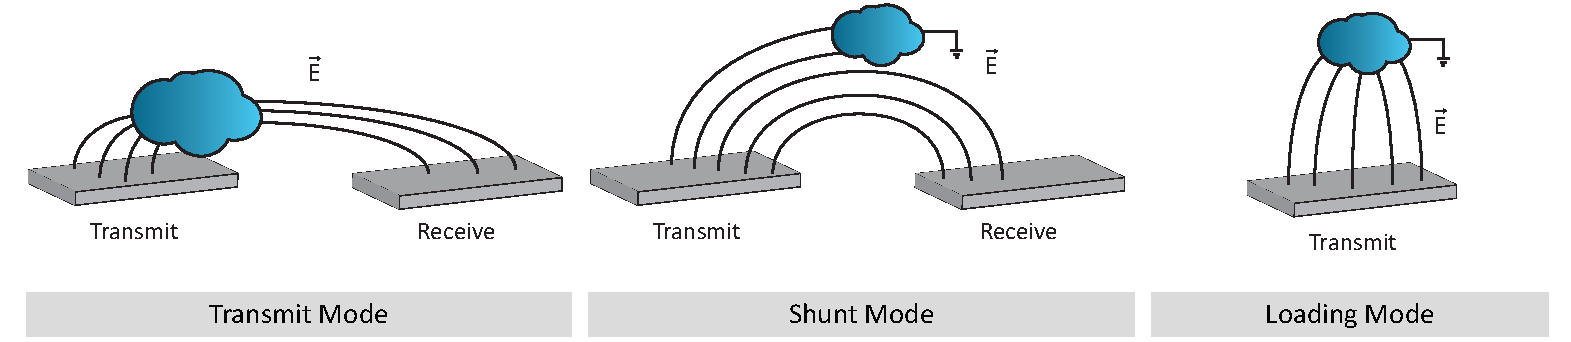
\includegraphics[width=1.00\textwidth]{Images/modes.pdf}
	\caption{Three different capacitive proximity sensing modes can be distinguished \cite{Smith1996}. The sensing electrodes build up an electric field to objects in the environment, illustrated with a cloud.}
	\label{fig:modes}
\end{figure}

In the field of capacitive proximity sensing, three different measurement modes (shown in Figure \ref{fig:modes}) were identified by Smith et al. \cite{Smith1999}: transmit mode, shunt mode and loading mode. Transmit mode is based on a varying electric potential coupled to an object that can be measured by a capacitive proximity sensor next to that object. Shunt mode applies two electrodes, a transmit and a receive electrode, that can measure capacitance changes produced by objects disturbing the electric field between the two electrodes. In loading mode, a single electrode builds up an electric field to any grounded object in the environment. By measuring the capacitance, conclusions can be made upon the proximity and nature of an object. In our work we apply loading mode since it requires only a single electrode that can be integrated invisibly into the wristband. 

Capacitive proximity sensing faces the great advantage of being robust against changing lighting conditions and occlusion. Moreover, sensing electrodes can be integrated invisibly into the environment. On the other hand, the exact distance to objects can only be approximated since the object's surface, its conductivity and grounding has influence on the measurement result. A single sensor will thus deliver data that has a certain degree of ambiguity. Due to the nature of capacitive proximity sensors, they can be prone to errors in environments with strong and rapidly changing electric fields. This, however, is usually not an issue when considering activities of daily living. 

A great variety of capacitive sensors and measurement techniques exists \cite{Smith1999}. The most common sensing principle, the loading mode, is based on running numerous charge and discharge cycles of the virtual capacitor that is created by the electrode and the environment. Depending on the charge and discharge times, one can infer the corresponding capacitance. This sensing principle is applied by Wimmer et al. in \cite{Wimmer2007} who presented a toolkit for capacitive proximity sensing. In previous works, capacitive proximity sensors were applied in various fields of human-computer-interaction. Wimmer et al. and Grosse-Puppendahl et al. presented gesture recognition systems \cite{Wimmer,Grosse-puppendahl2012} as well as smart furniture that can sense human activities \cite{Wimmer} and classify human postures \cite{Grosse-puppendahl2011}. Cheng et al. have investigated the possibility of using capacitive sensors for activity recognition by measuring shape changes of muscles and skin \cite{Cheng2010}. 
%To our knowledge, capacitive proximity sensors have not been embedded into a wearable device to enhance the performance of activity recognition.

\section{Hardware}
\label{sect:hardware}

This section presents the two components of our hardware prototype, the wrist-worn activity data logger tailored to capture acceleration data, and the capacitive proximity sensor used for distance measurements.

\subsection{Activity Data Logger}

The HedgeHog sensor \cite{hedgehog} is a custom designed wearable data logger aiming at long-term deployments in activity recognition scenarios. Due to its small form-factor (37x32x16mm) and weight, this wrist-worn sensor is an unobtrusive way to record relevant motion data.

%  (PIC18F46J50) (ADXL345) 

\begin{figure}[h]
	\centering
	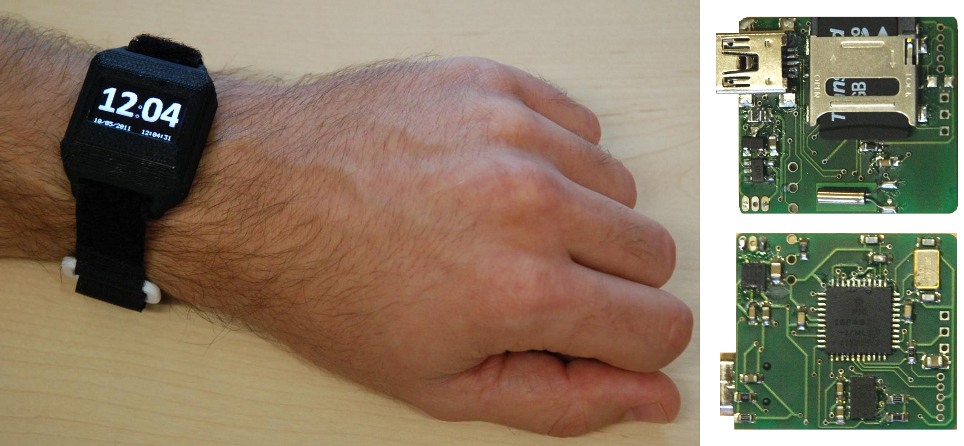
\includegraphics[width=\textwidth]{Images/hardware_sensor_2.jpg}
	\caption{The inertial data logger featuring a low-power microcontroller, a 3 axis accelerometer, a microSD flash card for storing the sensor data and a USB connector for accessing the data (on the right) is powered by a small lithium polymer battery and is packaged into a plastic case to be worn at the wrist (a version with an OLED display).}
	\label{fig:sensornode}
\end{figure}

The sensor node itself is built around the low-power Microchip microcontroller (PIC18F46J50) featuring an accelerometer sensor (ADXL345) to capture human motion, light and ambient temperature sensors and a microSD flash card for locally storing the sensor data. The sensor is powered by a $200mAh$ lithium polymer battery, which allows for two weeks of continuous recording on a single battery charge. A USB port is used to configure the sensor (e.g. setting the sensitivity of the accelerometer), to access the stored sensor data, and to recharge the battery. A plastic case packages and protects the sensor to be worn at the wrist (Figure \ref{fig:sensornode}).

The 3D accelerometer sensor is being sampled at 100Hz, resulting in 10ms equidistant measurements. For efficiency reasons, the sensor data is run-length encoded before being stored locally to the microSD card. 
The HedgeHog can be extended with further sensors tailoring different application scenarios. For our scenario, we have added a capacitive proximity sensor that is described in detail in the next section.



\subsection{Capacitive Proximity Sensor}

A wrist-worn capacitive proximity sensor requires a shield that eliminates the influence of the grounded arm directly underneath the sensor. Using this setup, we can detect the proximity to a grounded object in the environments for distances up to 20cm. Especially for mobile devices, it is required that the sensor draws a very small amount of power. Thus, other proximity sensing input modalities like ultrasound or optical measurements are not applicable for this type of mobile application.

The capacitive proximity sensor performs measurements in loading mode. Two electrodes are integrated into the wristband, one sensing electrode and one shielding electrode. The sensor draws a supply current of 1mA at 3.3V when active which qualifies it for wearable proximity sensing applications. In the following a virtual capacitor denotes the capacitance between the sensing electrode and the environment. The capacitance of the sensing electrode to environmental objects increases with closer distances.
% The capacitive proximity sensor performs measurements in loading mode. Two electrodes are integrated into the wristband, one sensing electrode and one shielding electrode that aims to eliminate the influence of the underlying skin. Without shielding no meaningful measurements could be performed, since the arm's skin is a very proximate grounded object to the sensing electrode. The sensor draws a supply current of 1mA at 3.3V when active and qualifies it for wearable proximity sensing applications. In the following a virtual capacitor denotes the capacitance between the sensing electrode and the environment. The capacitance of the sensing electrode to environmental objects increases with closer distances.

\begin{figure}[t]
	\centering
		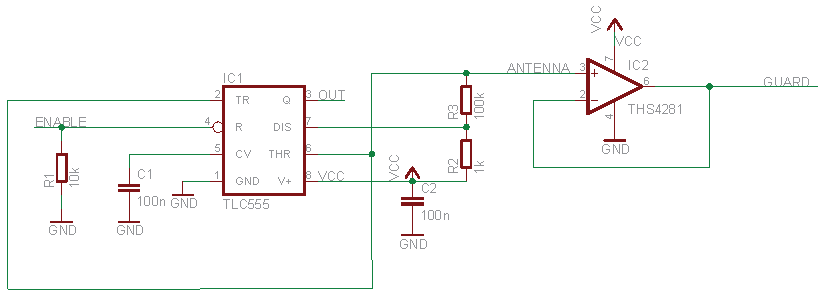
\includegraphics[width=1.00\textwidth]{Images/schematic.pdf}
	\caption{The sensing circuit is based on a timer with an operational amplifier that acts as a voltage follower. The wire that is labeled with ``antenna'' leads to the sensing electrode, whereas the wire labeled with ``guard'' leads to the shield electrode.}
	\label{fig:schematic}
\end{figure}

The sensing circuit schematic is shown in Figure \ref{fig:schematic}. It is based on a timer that controls the charging and discharging cycles of the virtual capacitor that is built by the sensing electrode and the surrounding environment. The timer toggles from charge to discharge at the time when a threshold voltage at the capacitor is reached. This results in an astable operation with succeeding charge/discharge cycles. When the capacitance of the virtual capacitor increases, the charging time will also increase and vice-versa.
Therefore, the capacitance is inversely proportional to the number of charging cycles in a given time span. In order to guard the sensor from measuring the capacitance to underlying objects, a shield electrode is placed directly underneath the measuring electrode. The shield is driven with the same potential as the sensing electrode, such that the capacitance between the two electrodes is negligible. Using this shielding method, the measured capacitance will only be slightly affected by the grounded underlying arm.

\begin{figure}[t]
	\centering
		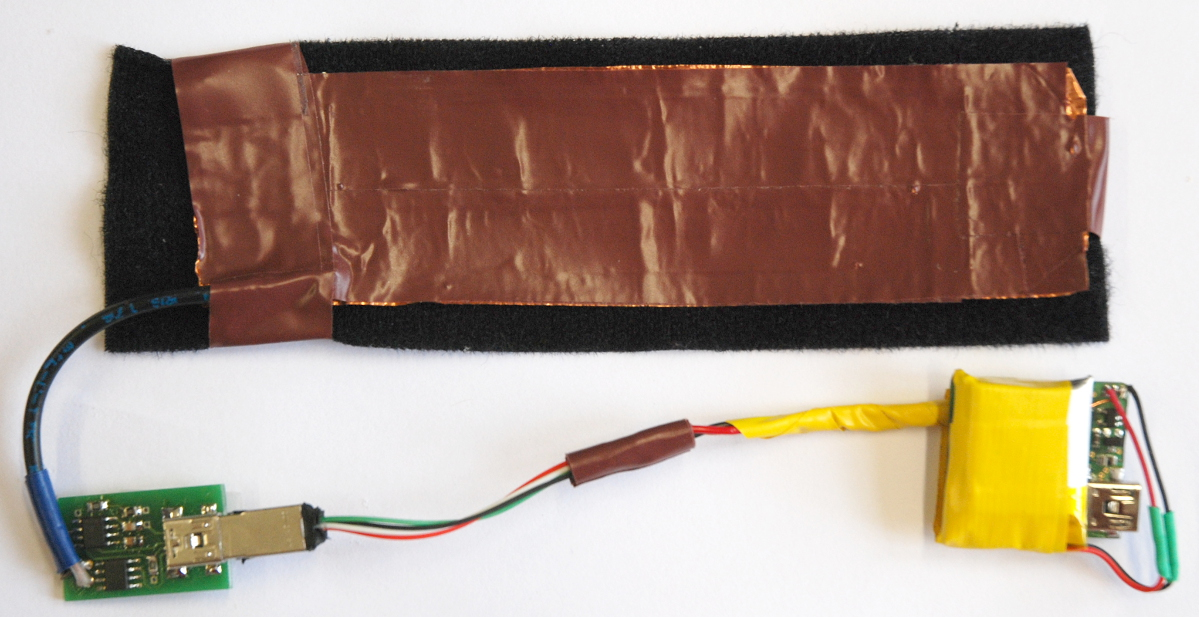
\includegraphics[width=\textwidth]{Images/capacitive_sensor_wristband_2.jpg}
	\caption{The hardware prototype at a glance: HedgeHog activity logger at the lower right, the capacitive sensor unit at the lower left, and the wristband with the sensing and the shield electrodes on-top each other. The electrodes are covered with adhesive tape for isolation purposes.}
	\label{fig:cap_sensor}
\end{figure}

\begin{figure}[t]
	\centering
 		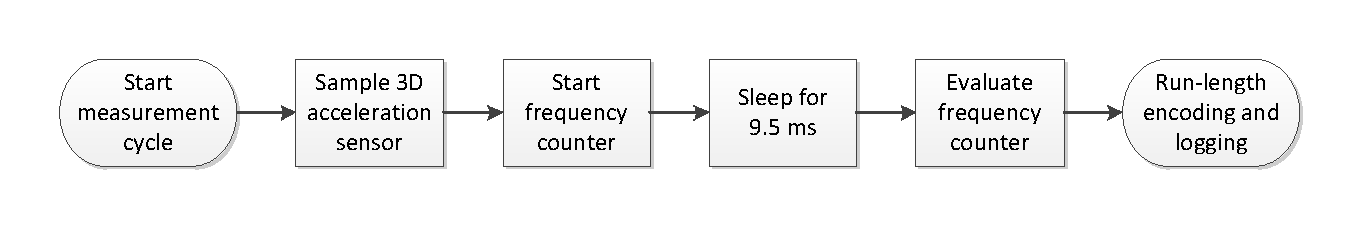
\includegraphics[trim=1cm 1cm 1cm 1cm,clip,width=\textwidth]{Images/pseudocode.pdf}
	\caption{Overview of the measurement procedure carried out by the HedgeHog sensor: using the microcontroller's Timer0 module in counting mode, the oscillating signal generated by the capacitive sensor circuit can be measured by counting the frequency pulses over a predefined gate time of approximately 9.5ms.}
	\label{fig:pseudocode}
\end{figure}


Figure \ref{fig:cap_sensor} shows the the wrist-worn prototype used in the evaluation experiments, with the HedgeHog as the main data logger, the capacitive sensor circuit and the wristband holding the sensing and shielding electrodes.

The operations required for a measurement cycle are illustrated in Figure \ref{fig:pseudocode}. The proximity sensor board generates a clock signal with varying frequency depending on the charge and discharge cycles. The HedgeHog measures the resulting capacitance by counting the signal's edges over a gate time of approximately 9.5ms. During that counting phase, the microcontroller is sent to sleep in order to reduce power consumption. 
%In the following, the HedgeHog applies run-length encoding on the measured data to reduce overhead and periodically logs the data to the integrated microSD card.

\section{Experiment}
\label{sect:experiment}

This section presents the experimental setup including the activities and the participants, as well as the findings that were obtained during the evaluation.

\subsection{Setup and Scenario}

The experiment setup aims to depict a typical scenario of a person in daily life. Especially in the field of Ambient Assisted Living (AAL), it is desired to monitor activities like drinking, preparing lunch and sleeping. A fine-grained monitoring of such activities may help elderly or people suffering from mental diseases to maintain a healthy day/night rhythm and take action if irregularities occur. Figure \ref{fig:cap_sensor} shows the modified HedgeHog activity logger that has been extended with a capacitive proximity sensor. The wristband has two electrodes, a sensing electrode underneath a slightly bigger shield electrode. 

The recorded test set contains the following activities: opening door, sitting on a couch, lying on a couch, putting kitchen equipments from a shelf and out of a locker, making a marmalade sandwich, eating the sandwich, pouring and drinking water, walking and sleeping. The relations of these activities to environmental objects are given in Table \ref{tab:activities}. Some of those activities are very hard to recognize when the data is limited to a single modality like a 3D accelerometer. For example, sitting at the table and sitting on a couch are very similar activities. We aim to show that the data basis can be significantly improved by the additional input modality. 

\begin{table}
	\centering
	\caption{Some details on the activities performed during the experiment and objects directly involved or nearby.}
	\setlength{\tabcolsep}{12pt}
	\begin{tabular}{lll}
		\toprule
		activities		& objects involved			& objects nearby			\\ 
		\midrule
		open door		& door knob 				& door  					\\
		sitting			& chair or couch			& body, chair, couch, table	\\
		lying			& couch						& body, couch, cushion		\\
		get things		& plate, glass, cutlery, 	& shelf, locker, fridge, table \\ 
						& bread, marmalade, bottle  & 							\\
		make sandwich	& bread, knife, marmalade	& table, plate 				\\
		eating			& marmalade sandwich		& table, plate, body		\\
		drinking 		& bottle, glass 			& table, body				\\
		sleeping		& bed, cushion, blanket		& body 						\\
		walking			& 							& body						\\
		 \bottomrule
	\end{tabular}
	\label{tab:activities}
\end{table}

In order to evaluate if capacitive proximity sensors in wrist-bands can enhance the performance of activity recognition, we have conducted an evaluation with 7 test persons. All test persons received a basic script with the activities they were supposed to perform. They were not given any instructions about the way they are supposed to perform the activities. After manual labelling, we used this test-set as ground truth and performed a 4-fold cross-validation on an support-vector machine (SVM) classifier on each user. The cross-validation was performed once with and once without including the data of the capacitive proximity sensor into the feature set. We chose an SVM classifier because of its high relevance in activity recognition and its fast performance. 

The classifier was trained with basic features that were extracted from a sliding window of 1 second width. Our first tests have shown that greater window sizes do not provide better classification results. In order to suppress noise contained in the capacitive proximity sensing data, we applied a moving average filter with a kernel size of 10. The final feature set contained the arithmetic mean, min, max, median and standard variance for each accelerometer axis and the capacitive proximity signal. These simple feature types represent standard features applied in activity recognition. Since we aim to show an improvement using the new modality, the selection of features and classifiers does not represent the primary focus of this paper. 

\subsection{Evaluation Results}
\label{sect:evaluation}

In the following, the performed activities will be analyzed in detail, stating the influence of the capacitive proximity sensor on the classification result. In general, the usage of data provided by the new modality showed improvements in recognition rates reaching from 2.4\% up to 10.7\% for single activities.

\begin{figure}[h]
	\centering
		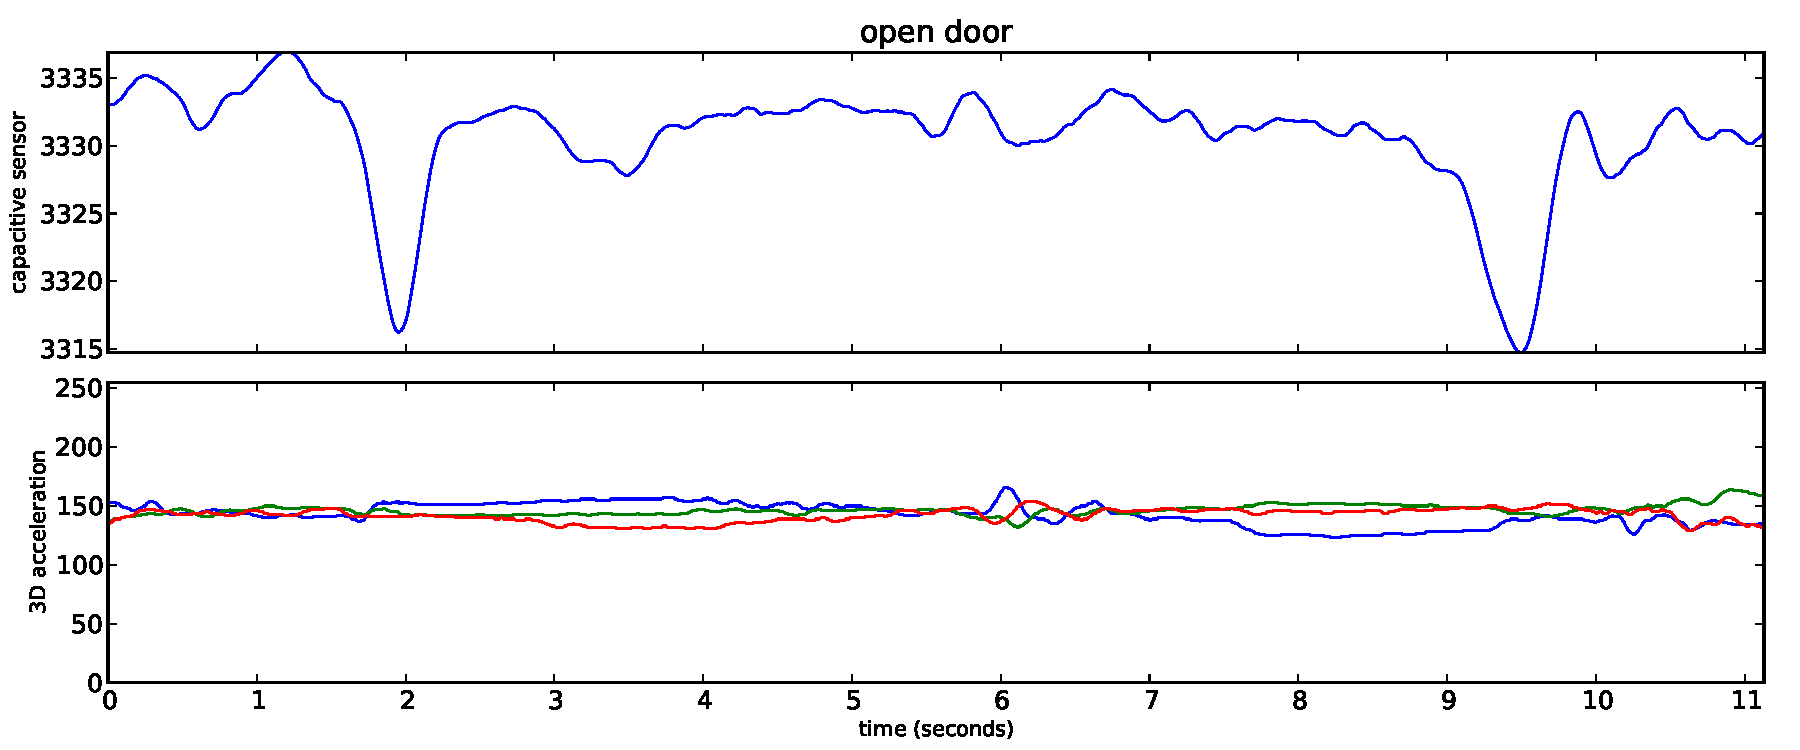
\includegraphics[width=1.00\textwidth]{../Auswertung/images/tobias_1.pdf}
	\caption{When the participants entered the apartment, the wrist approached the door knob twice, at the time of opening and closing the door. This fact can be observed in the capacitive proximity data (upper plot) at the beginning and at the end of the activity, whereas the acceleration has little characteristic information (bottom plot).}
	\label{fig:opendoor}
\end{figure}

The ''opening door'' activity has very poor recognition rates without the data from the proximity sensor. The average F-measure could be increased from 35.5\% to 46.2\%. A plot of the activity is given in Figure \ref{fig:opendoor}. The capacitive proximity sensor shows two approaches to the door knob, one for opening the door (2s) and one for closing the door (9s). The acceleration sensor captures relevant data in the time in which the person moves into the room and the hand changes from the outer to the inner door knob (5 - 7s). The recorded data for this activity also shows strong correlations between all experiment participants. The confusion matrices show that the ``open door'' activity was often confused with the ``sitting'' activity, probably because of the amount of motion on the one hand and the proximity to nearby objects (door, couch or cushions) on the other hand. By using the capacitive sensor data, the recall for that class and confusion with the sitting activity could be improved. 

\begin{figure}[h]
	\centering
		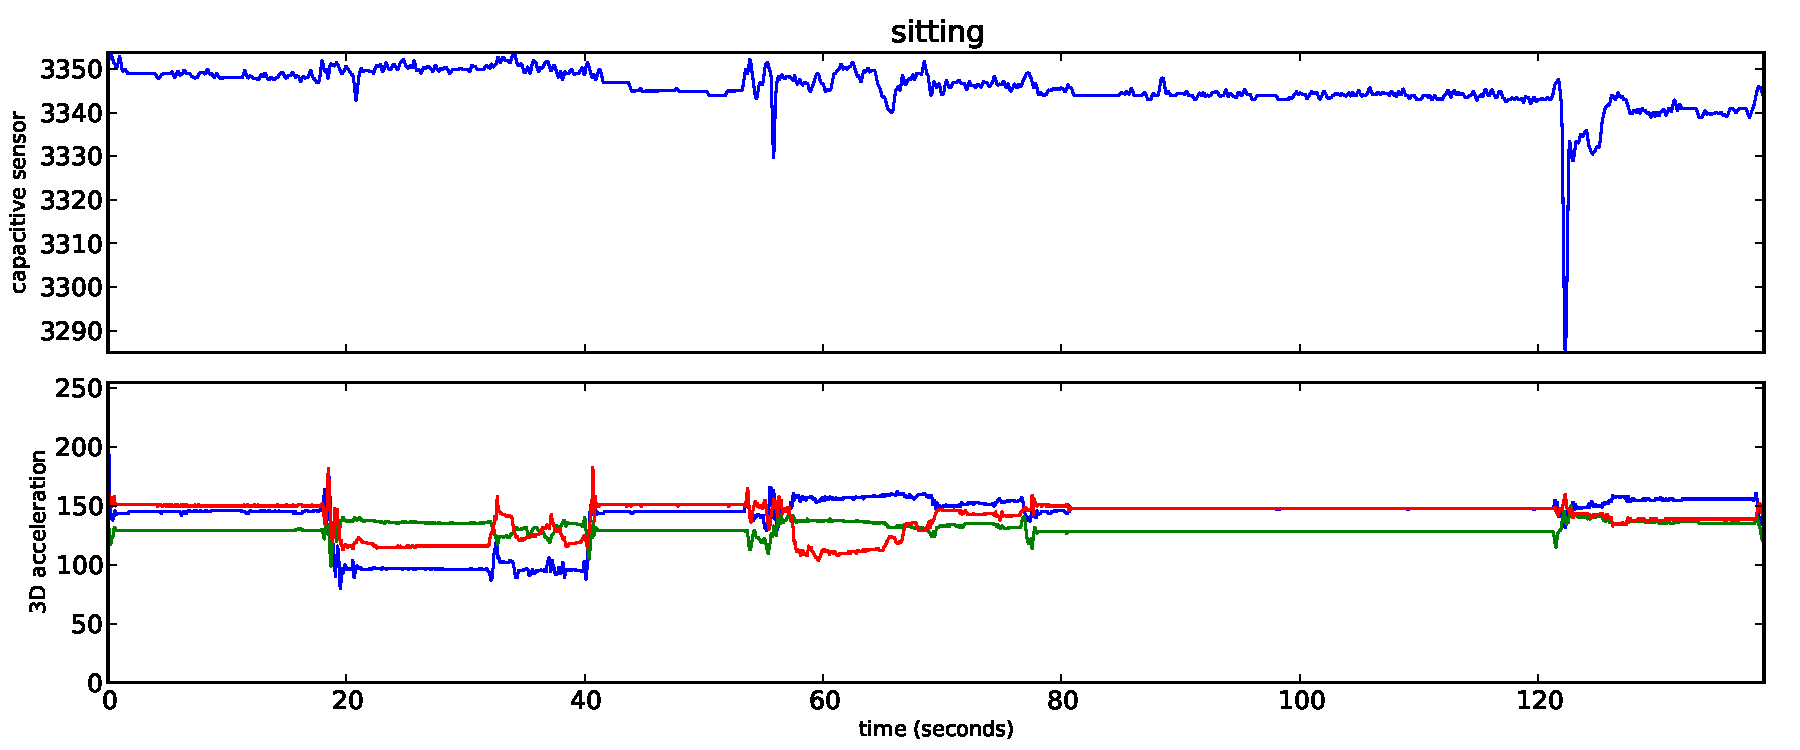
\includegraphics[width=1.00\textwidth]{../Auswertung/images/eugen_2.pdf}
	\caption{Example of the ``sitting'' activity in which the user moved his hands quite frequently (bottom plot). Most of the time the values of the proximity sensor stay more or less constant, probably due to the hands position on the couch's fabric. The sharp peak in the capacitive sensor data (upper plot) occurred when the participant scratched the back of his head. }
	\label{fig:sitting}
\end{figure}

After closing the door, the participants were supposed to sit down on the couch. It turned out that there are great variations of the sitting posture and the corresponding hand positions. Many users tapped with their fingers or hands while sitting, changed their sitting positions very frequently, or were even talking and gesticulating, as shown in Figure \ref{fig:sitting}. In this case, it is obvious that the data from the acceleration sensor is very difficult to interpret as there are numerous changes in the axial orientation of the sensor. However, the capacitive proximity sensor is able to indicate when a hand is placed on the surface of the couch. Especially for this particular participant, the F-measure increased from 50.3\% to 60.4\%, while the average F-measure improved from 68.0\% to 74.4\%. 

In the following, the participants were instructed to lie  down on the couch. Again, there were great variations in how this activity was performed by the participants. For example, some of them crossed their hands under their head, or placed them on their body. For this class, the average F-measure could only be increased by 2.4\%, from 81.2 to 83.6\%. Considering some participants, the activity was often confused with the ``make sandwich'' class. By using the proximity modality, the confusion between the two classes could be reduced.

\begin{figure}[t]
	\centering
		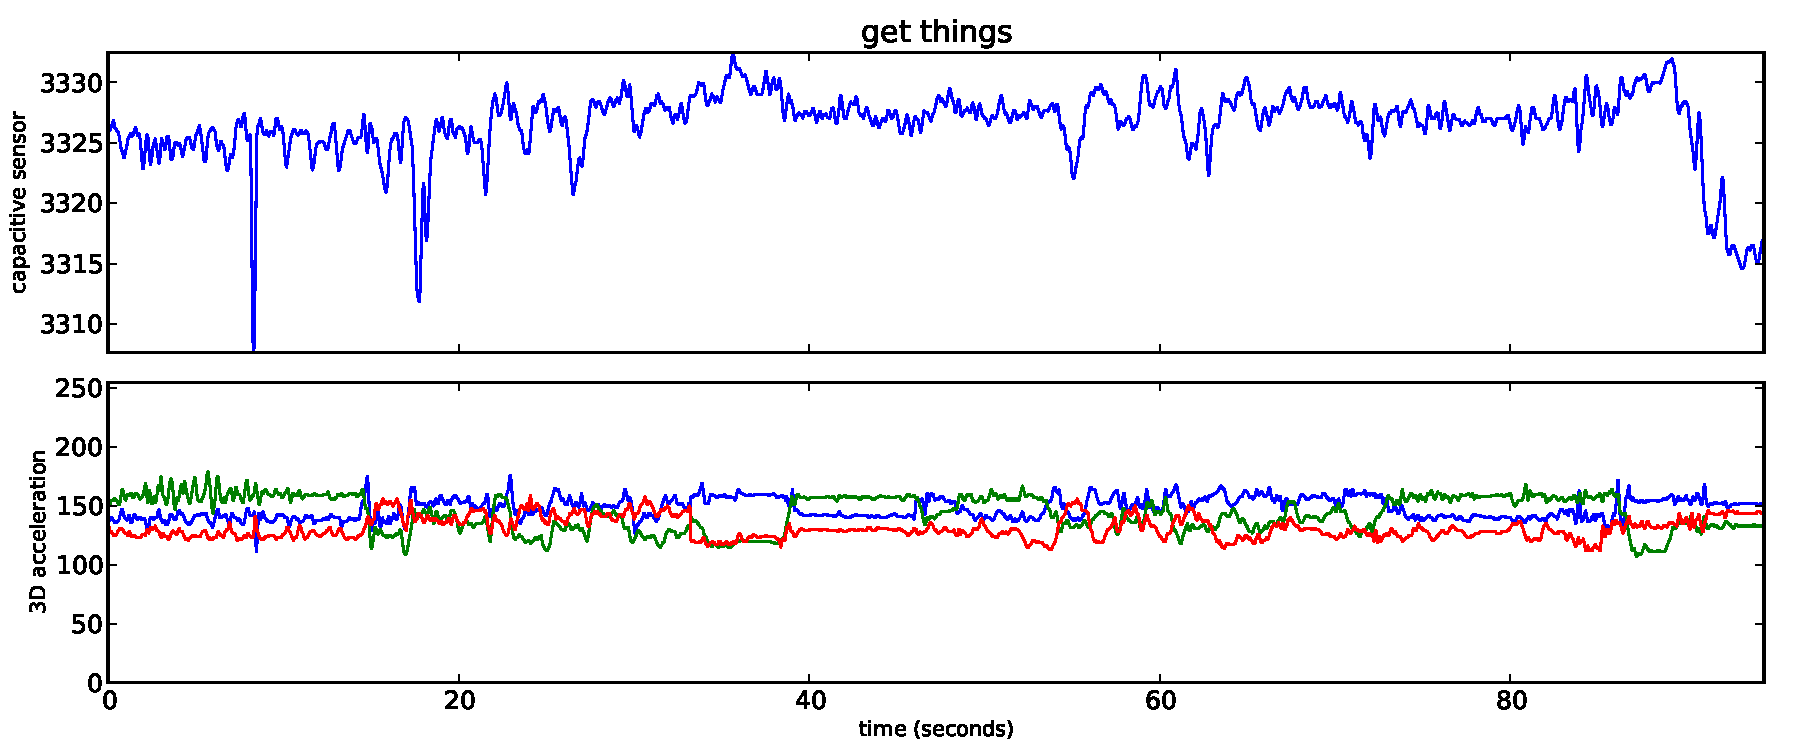
\includegraphics[width=\textwidth]{../Auswertung/images/tobias_4.pdf}
	\caption{An example of the ``get things'' activity, where the participants had to get food and dishes from shelves and lockers. The proximity sensor peaks in the beginning (9s and 19s) indicate immediate proximity to shelf, and to the locker (55-63s) in the kitchen (upper plot). The signal drop at the end results from the participant placing his hand on the table when she was finished.}
	\label{fig:get_things}
\end{figure}

After that, the participants were asked to walk over to the kitchen and to put food and dishes from a shelf and a locker on the table. This activity involved direct interactions with various objects as well as proximity to furniture in the room (see Table \ref{tab:activities}). The capacitive proximity sensor was able to capture the proximity to the shelf and to the table (see Figure \ref{fig:get_things}). The average F-measure for this activity is rather low, but improved by 6.8\% from 53.8\% to 60.6\%. 
The worst performing participants for this activity reached an F-measure of 46.8\% without and 53.5\% with the capacitive sensor, while the best performing one reached 62.0\% and 64.5\% respectively. The low performance results from confusions with other activities, with a higher tendency to the ``make sandwich'' activity across all participants. This is most likely due to various objects involved in both activities, and the fact that 1-second features are obtained. The capacitive sensor modality has a more positive impact reducing the confusion with other activities.

\begin{figure}[h]
	\centering
		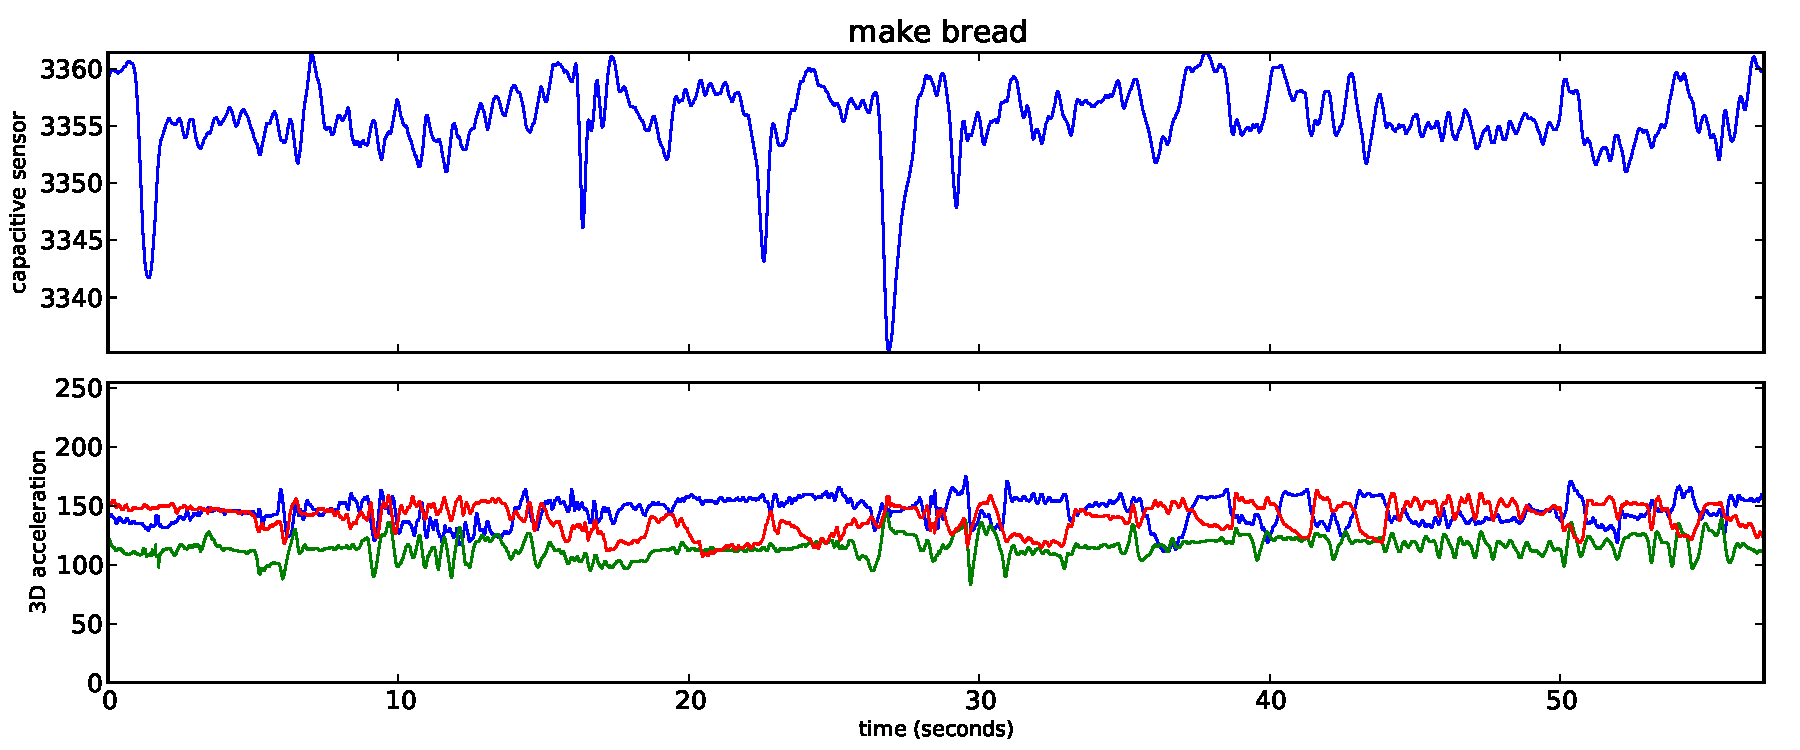
\includegraphics[width=\textwidth]{../Auswertung/images/eugen_5.pdf}
	\caption{An example of the ``make sandwich'' activity, where the participants had to put marmalade on a slice of bread. The proximity sensor indicates the closeness to the table, while the acceleration sensor shows recurring hand motions.}
	\label{fig:prep_bread}
\end{figure}

Figure \ref{fig:prep_bread} shows an example instance of preparing a bread with marmalade. It is notable that the acceleration data does not seem to provide any characteristic patterns, while the proximity sensor indicates a table, plate, or other objects in immediate distance. This activity showed a high improvement in the average F-measure by 10\%, from 49.0\% to 59.8\%, where the data delivered by the capacitive proximity sensor is taken into account. The ''make sandwich'' class was often confused with the ''sitting'' class for some users, probably due to lots of motion during the sitting, as mentioned previously. For other users, ''make sandwich'' was confused with ''eating'' or ''drinking''. Using the new input modality, confusion across users could be reduced.

\begin{figure}[h]
	\centering
		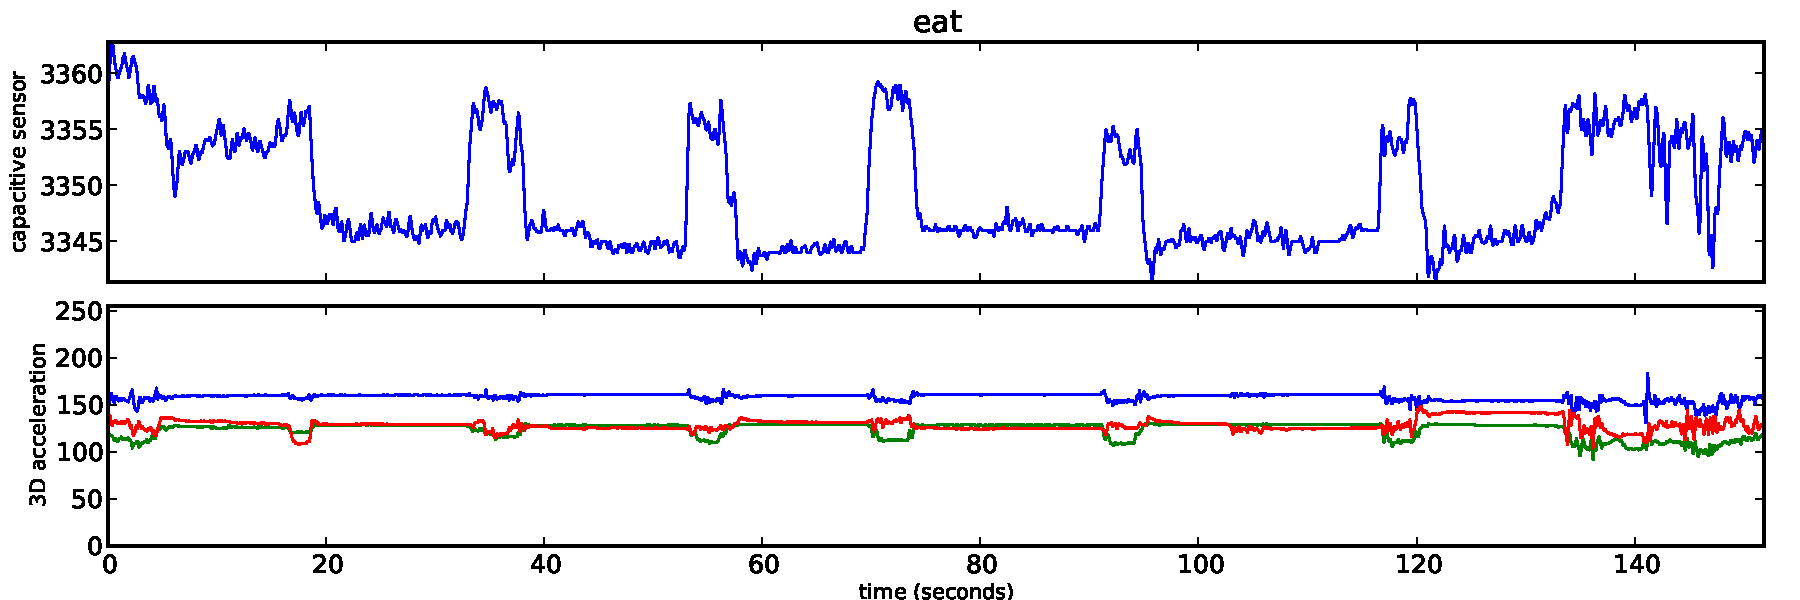
\includegraphics[width=\textwidth]{../Auswertung/images/eugen_6.pdf}
	\caption{An example of a participant eating a marmalade sandwich, taking 5 bites from it. After each bite, the hand is placed on the table, which can be recognized both in the acceleration as well as the proximity data plots.}
	\label{fig:eating}
\end{figure}

When considering the eating activity, the impact of the new capacitive proximity sensor on the classification performance is quite low, as the chosen features are able to distinguish it from other activities. Some of the participants ate their sandwich leaving their hand close to the mouth, while others moved their hand up and down putting their sandwich aside on the plate, which also results in the performance range from 71.2 to 88.1\% without and 77.5 to 90.6\% with the proximity data. An example of an eating activity is shown in Figure \ref{fig:eating}, where the participant took a few bites from the sandwich while putting it down every time. The average F-measure increased slightly by 2.7\% (from 79.5\% to 82.2\%). 

\begin{figure}[t]
	\centering
		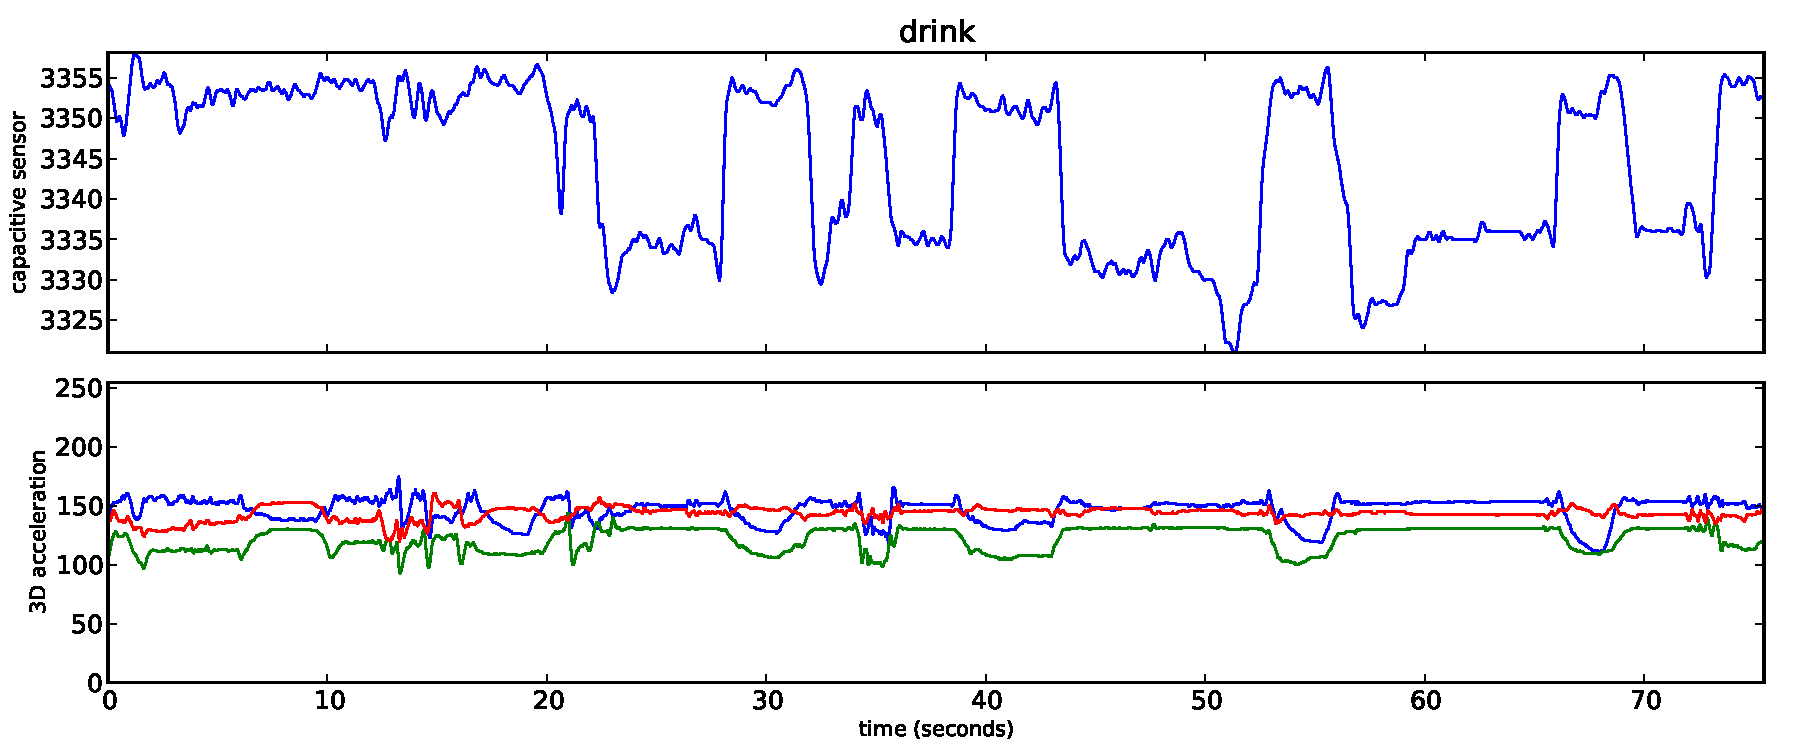
\includegraphics[width=\textwidth]{../Auswertung/images/eugen_7.pdf}
	\caption{An example of the ``drinking'' activity. The participant first pours some water into the glass and then takes three drinks of water. After each sip, he returns his arm to the table which can be observed in the characteristic patterns of the proximity sensor.}
	\label{fig:drinking}
\end{figure}

The activity ``drinking water'' is depicted in Figure \ref{fig:drinking}. The participant took a few sips from the glass, with leaving the hands positioned. These motions can be easily detected in the acceleration as well as proximity data. The accelerometer data shows that there periodic up- and down-movements while the capacitive proximity sensor delivers data that is associated to the proximity of the table. The F-measure lies at 48.4\% without and 54.4\% with the proximity data taken into account, resulting in a gain of 6\%.

\begin{figure}[t]
	\centering
		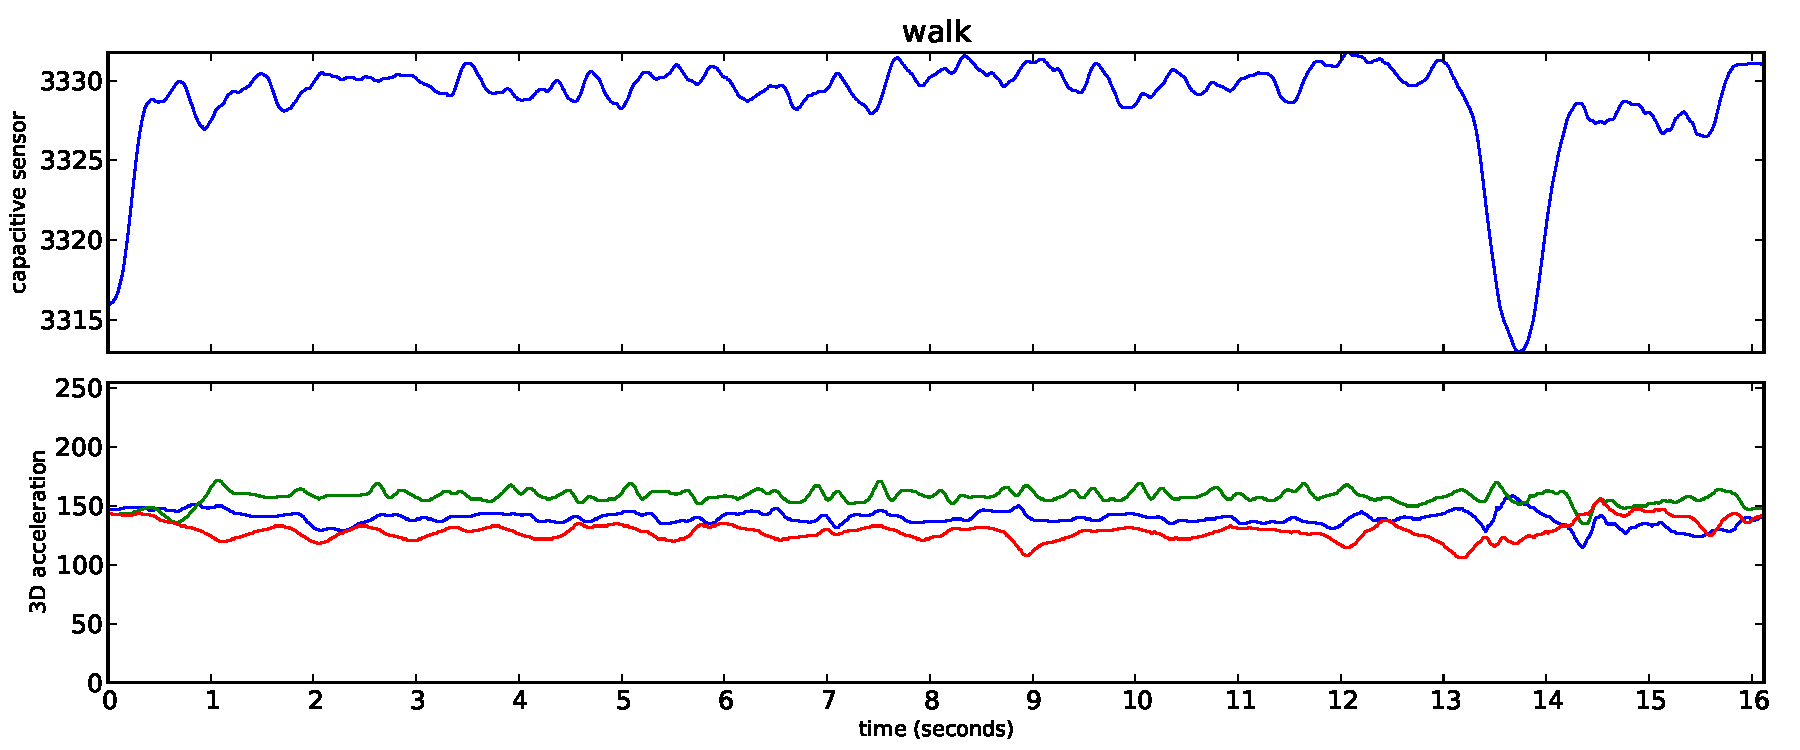
\includegraphics[width=1.00\textwidth]{../Auswertung/images/marko_8.pdf}
	\caption{An exemplary instance of the class ``walking''. The acceleration sensor and the proximity sensor show periodic recurring patterns that are related to the pendulum-like arm movement and the proximity to the person's body during those movements.}
	\label{fig:walking}
\end{figure}

Regarding the walking activity one can identify periodic changes in the acceleration as well as in the measured capacitance, illustrated in Figure \ref{fig:walking}. While walking, the capacitance between the wristband and the leg increases when the wristband is located close to the body and decreases when the wristband moves away. There were problems distinguishing this activity from ``get things'' that could be improved by using the new input modality. The classification improvement for this activity accounts to 12.2\% boosting the average F-measure from 41.7\% without to 53.9\% with the new sensor. Due to the low performance results and the characteristic periodic signal shape, it would help to consider frequency domain features, as it is often applied in related work.

\begin{figure}[t]
	\centering
		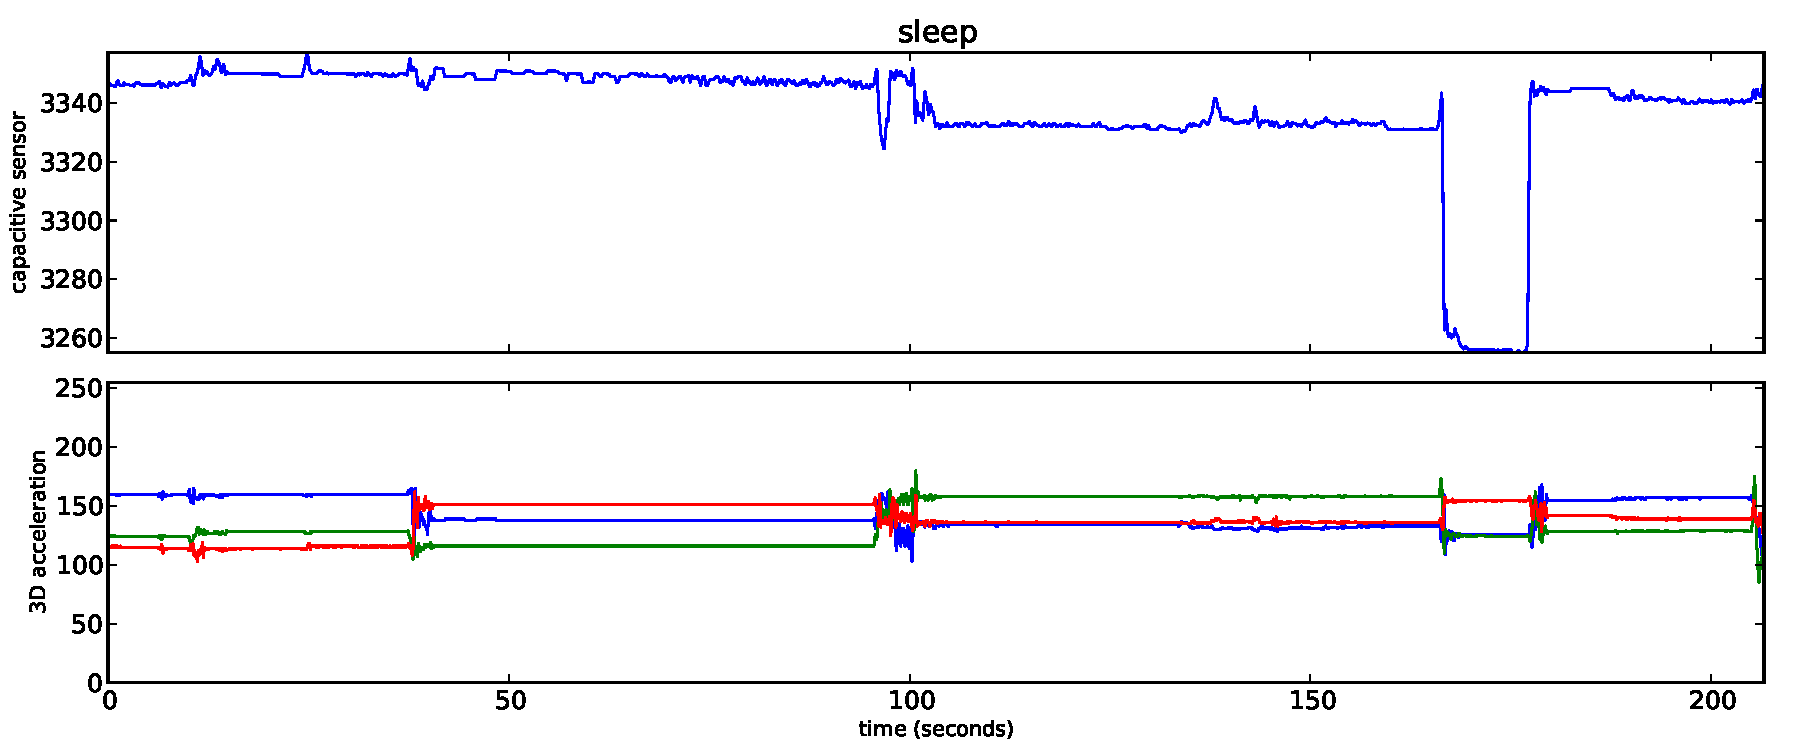
\includegraphics[width=1.00\textwidth]{../Auswertung/images/eugen_9.pdf}
	\caption{During the sleeping activity the data from both sensors remains constant for large time spans. The capacitive sensor plot shows the coverage of the arm with either cushions, blankets or the proximity to the mattress, other parts of the bed, the head or body of the participant.}
	\label{fig:sleeping}
\end{figure}

The sleeping activity (an example shown in Figure \ref{fig:sleeping}) was classified with an average F-measure of 83.2\%, which increased to 86.9\% when using the proximity data. In this case, the capacitive proximity sensor is able to capture the surrounding cushions and blankets, as well as the body or head of the participant. The accelerometer data and the capacitive proximity data have larger periods of low variance, which is a cause for confusion with the ``lying on the couch'' activity.

\begin{figure}[t]
	\setlength{\tabcolsep}{1.7pt}
	\centering
	\begin{scriptsize}
	\begin{tabular}{|ccccccccc|p{0.01cm}|ccccccccc|p{0.01cm}|l}
% 		\toprule
		\multicolumn{9}{c}{without proximity data} &\multicolumn{1}{c}{}& 
			\multicolumn{9}{c}{with proximity data} &\multicolumn{1}{c}{}&  \\ \cmidrule{1-9} \cmidrule{11-19} 
			
		\multicolumn{1}{c}{a} & b & c & d & e & f & g & h & \multicolumn{1}{c}{i} &\multicolumn{1}{c}{}& 
			\multicolumn{1}{c}{a} & b & c & d & e & f & g & h & \multicolumn{1}{c}{i} 	&\multicolumn{1}{c}{}& $\leftarrow$ classified as\\
		\cline{1-9} \cline{11-19} \cline{21-21}
\textbf{8} & 0 & 0 & 0 & 0 & 0 & 0 & 2 & 1		&& \textbf{11} & 0 & 0 & 2 & 1 & 0 & 0 & 0 & 1 	&& a = open door	\\ 
0 & \textbf{140} & 0 & 5 & 2 & 0 & 0 & 0 & 0  	&& 0 & \textbf{140} & 0 & 5 & 2 & 0 & 0 & 0 & 0 && b = sitting		\\ 
0 & 0 & \textbf{294} & 1 & 9 & 10 & 1 & 1 & 0 	&& 0 & 0 & \textbf{309} & 1 & 0 & 4 & 0 & 0 & 1 && c = lying		\\ 
1 & 7 & 1 & \textbf{50} & 17 & 9 & 1 & 4 & 1	&& 2 & 6 & 0 & \textbf{67} & 14 & 9 & 1 & 2 & 1 && d = get things	\\ 
0 & 2 & 7 & 7 & \textbf{102} & 42 & 5 & 0 & 2	&& 1 & 1 & 0 & 13 & \textbf{120} & 24 & 7 & 1 & 1&& e = make sandwich	\\ 
0 & 0 & 3 & 5 & 21 & \textbf{288} & 4 & 0 & 0 	&& 0 & 0 & 2 & 1 & 19 & \textbf{300} & 3 & 0 & 0 && f = eating		\\ 
0 & 5 & 11 & 1 & 29 & 40 & \textbf{18} & 0 & 0	&& 0 & 4 & 4 & 0 & 26 & 57 & \textbf{16} & 0 & 0 && g = drinking	\\
2 & 0 & 0 & 2 & 0 & 0 & 0 & \textbf{11} & 0	 	&& 2 & 0 & 0 & 0 & 0 & 0 & 0 & \textbf{14} & 0 	 && h = walking		\\
0 & 2 & 2 & 0 & 2 & 0 & 0 & 0 & \textbf{271}	&& 0 & 0 & 0 & 0 & 1 & 0 & 0 & 0 & \textbf{276}  && i = sleeping	\\ 
		\cline{1-9} \cline{11-19} 
% 		\bottomrule
	\end{tabular}
	\end{scriptsize}
	
	\caption{Activity recognition evaluation revealing the positive impact of the capacitive proximity sensor. Here, we are comparing SVM classification presented as confusion matrices for an exemplary user, without the proximity data on the left, and with the proximity data on the right. Note that the reject class (background data not annotated as an activity) is not included in the confusion matrix.}
	\label{fig:ConfusionMatrixForAnExemplaryUser}
\end{figure}

Figure \ref{fig:ConfusionMatrixForAnExemplaryUser}  depicts two confusion matrices for an exemplary participant from our evaluation, once without and once with including the proximity data. In most activities, an enhancement in the number of correctly classified instances is observable. The ``lying'' activity's recognition performance could benefit a lot from the proximity data, improving both precision and recall. 

A better classification performance can also be observed for the ``get things'' class that includes interactions with a multitude of objects in the environment. Regarding the activity ``make sandwich'', the capacitive proximity could reduce the number of confusions with the ``eating'' class significantly.

Due to the high similarity of eating and drinking (cf. Figure \ref{fig:eating} and \ref{fig:drinking}), the number of confusions between those two classes increases when considering the proximity data. However, for the ``drinking'' class the new modality limits the confusions to related activities such as ``eating'' and ``make sandwich'' only, while lowering the number of false recognitions for the other activities.

\section{Conclusion and Outlook}
\label{sect:conclusions}

Our paper presented a wrist-worn activity data logger prototype, which consists of an accelerometer in combination with a capacitive proximity sensor integrated into the wristband. Our experiments with seven participants and nine daily activities show that this additional input modality can significantly boost the activity recognition performance.
Regarding the classification performance, we obtained an improvement in the average F-measure of 6.3\%, from 67.2 to 73.5\%. Specifically, the activity classes ``walking'', ``make sandwich'' and ``open door'' could benefit a lot from proximity-related sensor data. For such classes, the classification performance could be boosted by 12.2\%, 9.0\% and 10.8\% respectively. 

With this proof of concept we show that the proximity information can provide an information gain regarding the evaluated activities. In future work we aim at evaluating other relevant feature types, such as frequency domain features, as well as feature sets to extract the most discriminative ones. Additionally, using other classifiers (such as HMMs) might also improve activity recognition performance.

The classification results could also be improved by using more than one sensing electrode in the wristband. For example, the wristband could integrate up to four electrodes that are placed on each side of the arm. However, this will lead to smaller electrode surfaces thus resulting in a decreased sensing distance. The sensor's power consumption can be decreased by shorter measurement windows and the choice of more energy efficient hardware components as well as software implementation. Measuring pulse width lengths instead of counting the number of pulses of the sensor's signal may reduce the required time needed for a measurement, thus increasing the time the microcontroller is able to sleep.

Capacitive proximity sensors represent a suitable new input modality for future activity recognition systems. The low power consumption as well as the unobtrusive integration of a sensor into the wristband meets an essential requirement of wearable applications. Especially in AAL environments, these systems can help monitoring the course of chronic diseases by recognizing activities of daily life. This may improve the quality of life of persons affected and their caregivers. 

\section*{Acknowledgements}

We would like to thank our evaluation participants from the Technische Universit\"at Darmstadt and Fraunhofer IGD.

\bibliographystyle{splncs03}
\bibliography{references}

\end{document}
